
%EXCERCISE 2 :)

\section{\color{olive}Excercise 2: State Machines to Detect the sequence 1-1-0-1}
In this exercise, the detection of the sequence 1-1-0-1 inside a longer sequence of bits, is done with a Moore's state machine and with a Mealy's state machine. The main difference between these two state machines is that in Moore's one, the output only depends on the present state of the machine, while in Mealy's one, the output depends on the present state as well as on the input. This causes a time displacement between the output of both state machines. Moore's output "answers" to the input one clock later after having reached the new state, while Mealy's output "answers" immediatly during the same clock that the input arrives. This is because Mealy's reacts not only according to the present state, but also depending on the input's value.

For the implementation of both state machines, five states are needed and they are represented with the letters from A to E:\\ 
- A (000): "IDLE", the state in which the first digit of the sequence has not yet been detected.\\
- B (001): The first digit of the sequence, "1", has arrived.\\
- C (010): The second digit of the sequence, "1",  has arrived.\\
- D (011): The third digit of the sequence, "0", has arrived.\\
- E (100): The last digit of the sequence, "1", has arrived.\\ \\
The states are digitally represented with three bits, as they allow to get five different combinations, so that the name of each state is represented with a binary number. Such representation is the one given between parenthese, after the name of each state.  It is important to mention that no matter which is the present state, whenever a "0" arrives from reset, the state changes to state A (IDLE). 

\subsection{\color{purple}Moore's Type State Machine}

In figure \ref {MOOREFSM} it is represented the sequence detection with the Moore's state machine.

\begin{figure}[H]
\centering
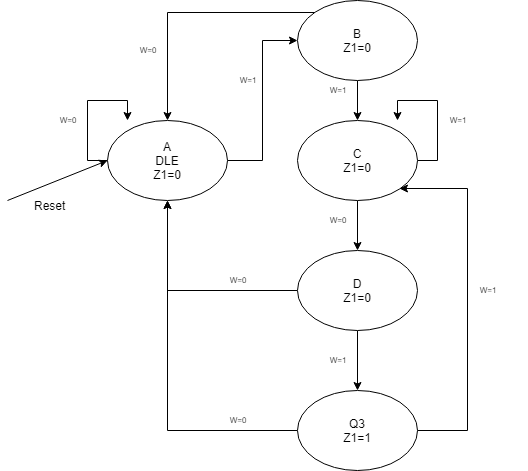
\includegraphics[scale=0.5]{../Exercise2/EJ2MOORE}
\caption{\color{cyan}Moore's State Machine, for detecting the sequence 1-1-0-1.}
\label{MOOREFSM}
\end{figure}

From above's diagram (the one in figure \ref {MOOREFSM}), the following table \ref {measej1} is obtained. 
\begin{table}[H]
\begin{center}
\begin{tabular}{|c|c c c|c|}
\hline
Present State & & Next State & & Output z \\
 & &depending on w & &  \\
 & w=0 & & w=1 &   \\
\hline
\hline
A  (000) & A (000)& & B (001)& 0   \\
\hline
B (001)& A (000)& & C(010) & 0   \\
\hline
C (010)& D (011)& & C (010)& 0   \\
\hline
D (011)& A (000)& & E (100& 0   \\
\hline
E (100)& A (000)& & C (010)& 1   \\
\hline
\hline
\end{tabular}
\end{center}
\caption{\label{measej1}\color{cyan}Moore's Next States and Outputs.}
\end{table}

The way the reset influences is not shown in the tables because it works the same way for it ocurring at any of the states. If reset=1, nothing happens. But if it equals 0, the reset occurs. It works as a negative reset. Apart from that, the present state is represented as a 3 bit vector y: (y3,y2,y1) while the next state is represented as Y: (Y3,Y2,Y1). From the previous table \ref {measej1} the following Karnaugh maps are used to get to simple logic expressions. The first Karnaugh map is to get Y1, the second one for Y2, the third one for Y3 and the last one for the output z. As three bits are being used to represent the states, there are combinations of these bits that act as don't cares (x) in the Karnaugh maps. This is because we have only five states, and three bits give more than five combinations. This helps simplifying even more the final expressions.

\begin{center} 
        \begin{Karnaugh}
            %cada 4 es una fila, la col 3 es la 4ta columna y 3fila es la 4 fila
            \contingut{
            0,0,1,0,
            0,X,X,X,
            1,0,0,0,
            0,X,X,X}
            \implicant{2}{6}{red}
            \implicant{8}{8}{green}
%            \implicant{12}{8}{orange}
%            \implicantdaltbaix[3pt]{1}{9}{blue}
            %\implicantcantons[2pt]{orange}
            %\implicantcostats{4}{14}{green}
        \end{Karnaugh}
    \end{center}



\begin{center}
        \begin{Karnaugh}
            %cada 4 es una fila, la col 3 es la 4ta columna y 3fila es la 4 fila
            \contingut{
            0,0,1,0,
            0,X,X,X,
            0,1,1,0,
            1,X,X,X}
            \implicant{2}{10}{red}
            \implicant{12}{14}{green}
%            \implicant{12}{8}{orange}
            \implicant{13}{9}{blue}
%            \implicantdaltbaix[3pt]{1}{9}{blue}
            %\implicantcantons[2pt]{orange}
            %\implicantcostats{4}{14}{green}
        \end{Karnaugh}
    \end{center}
  
  
\begin{center}
        \begin{Karnaugh}
            %cada 4 es una fila, la col 3 es la 4ta columna y 3fila es la 4 fila
            \contingut{
            0,0,0,0,
            0,X,X,X,
            0,0,0,1,
            0,X,X,X}
            \implicant{15}{11}{red}
%            \implicant{12}{14}{green}
%%            \implicant{12}{8}{orange}
%            \implicant{13}{9}{blue}
%            \implicantdaltbaix[3pt]{1}{9}{blue}
            %\implicantcantons[2pt]{orange}
            %\implicantcostats{4}{14}{green}
        \end{Karnaugh}
    \end{center}
    
   
    \begin{center}
        \begin{Karnaughvuit}
            %cada 4 es una fila, la col 3 es la 4ta columna y 3fila es la 4 fila
            \minterms{4}
        \maxterms{0,1,2,3}
        \indeterminats{5,6,7}
            \implicant{4}{6}{red}
%            \implicant{12}{14}{green}
%%            \implicant{12}{8}{orange}
%            \implicant{13}{9}{blue}
%            \implicantdaltbaix[3pt]{1}{9}{blue}
            %\implicantcantons[2pt]{orange}
            %\implicantcostats{4}{14}{green}
        \end{Karnaughvuit}
    \end{center}

From the Karnaugh maps, we get to the following expressions:
$$Y1 = \overline{y1} (\overline{y2}   \overline{y3}  w + y2 \overline{w})$$
$$Y2 = y2  \overline{y1} + w (y3 + \overline{y2}  y1)$$
$$y3 = y1  y2  w $$
$$z = y3 $$

These expressions lead to the following circuit, shown in figure \ref{ej2circuit}:

\begin{figure}[H]
\centering
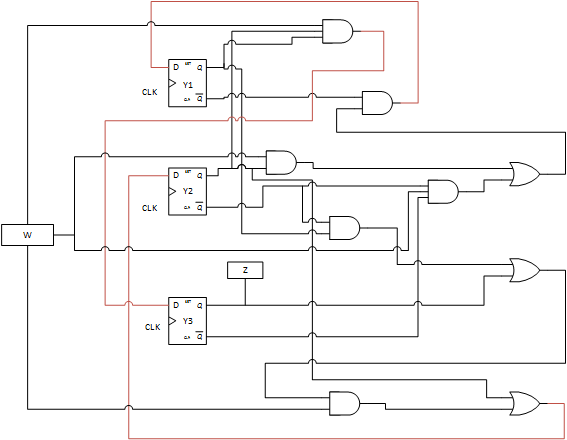
\includegraphics[scale=0.8]{../Exercise2/ej2circuit}
\caption{\color{cyan}Logical circuit for the Moore's state machine.}
\label{ej2circuit}
\end{figure}

The previous figure  \ref {ej2circuit} shows how the present state is saved using the three D flip-flops, each saving one of the bits that form the represented state's value.

\subsubsection{\color{orange}Coding and testing of the Moore's State Machine}
This state machine was written in verilog, considering the previous state and deciding what state whould come next, according to the input. In this case, each state has an output associated. The code was tested using a 64-bit sequence arriving to the state machine through the input. This sequence considers the different cases for the detection of the sequence and the cases in which it should go back to the IDLE state. Two different tests were carried out. One of them without resetting the state machine, in order to check the correct functioning of the transitions among states. The other test was made using the same input sequence, and adding another reset sequence, in which the reset response to a reset is tested in all of the states. The tests are clearly seen using gtkwave, and the results are shown bellow in figures \ref{gtk} and \ref{gtkr}.


\begin{figure}[H]
\centering
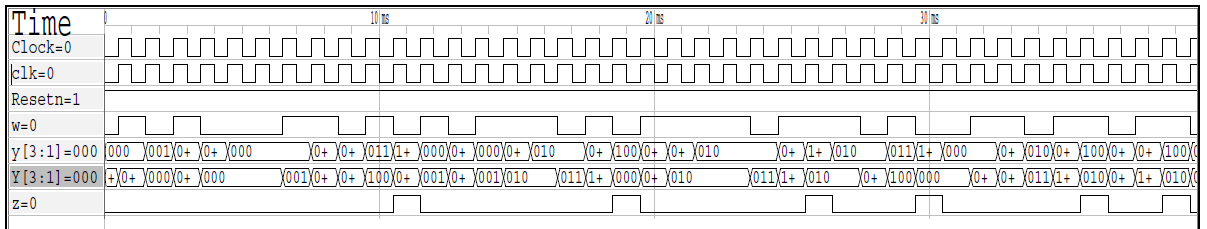
\includegraphics[scale=0.9]{../Exercise2/Moore/gtk0}\\ 
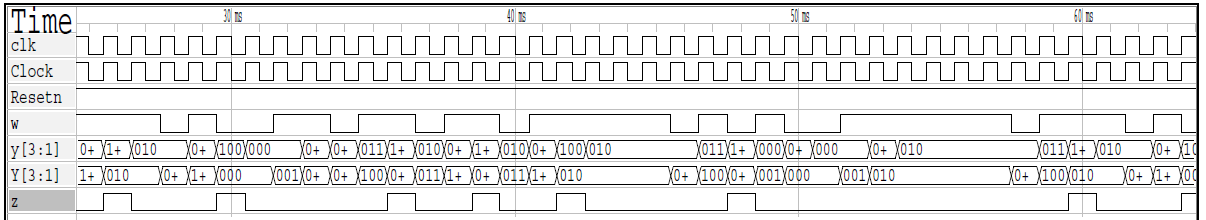
\includegraphics[scale=0.9]{../Exercise2/Moore/gtk11}
\caption{\color{cyan}Test of Moore's State Machine without resetting.}
\label{gtk}
\end{figure}

\begin{figure}[H]
\centering
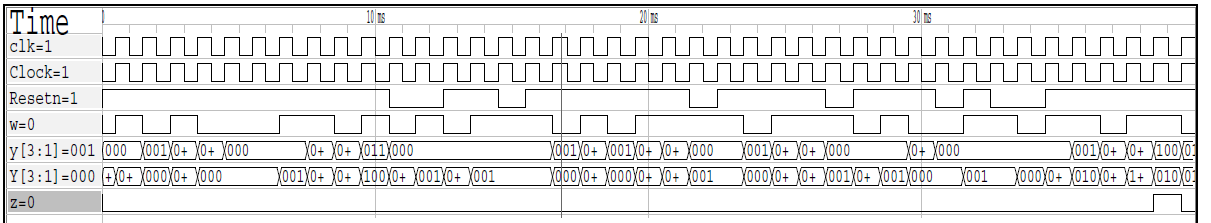
\includegraphics[scale=0.9]{../Exercise2/Moore/gtkr1}\\
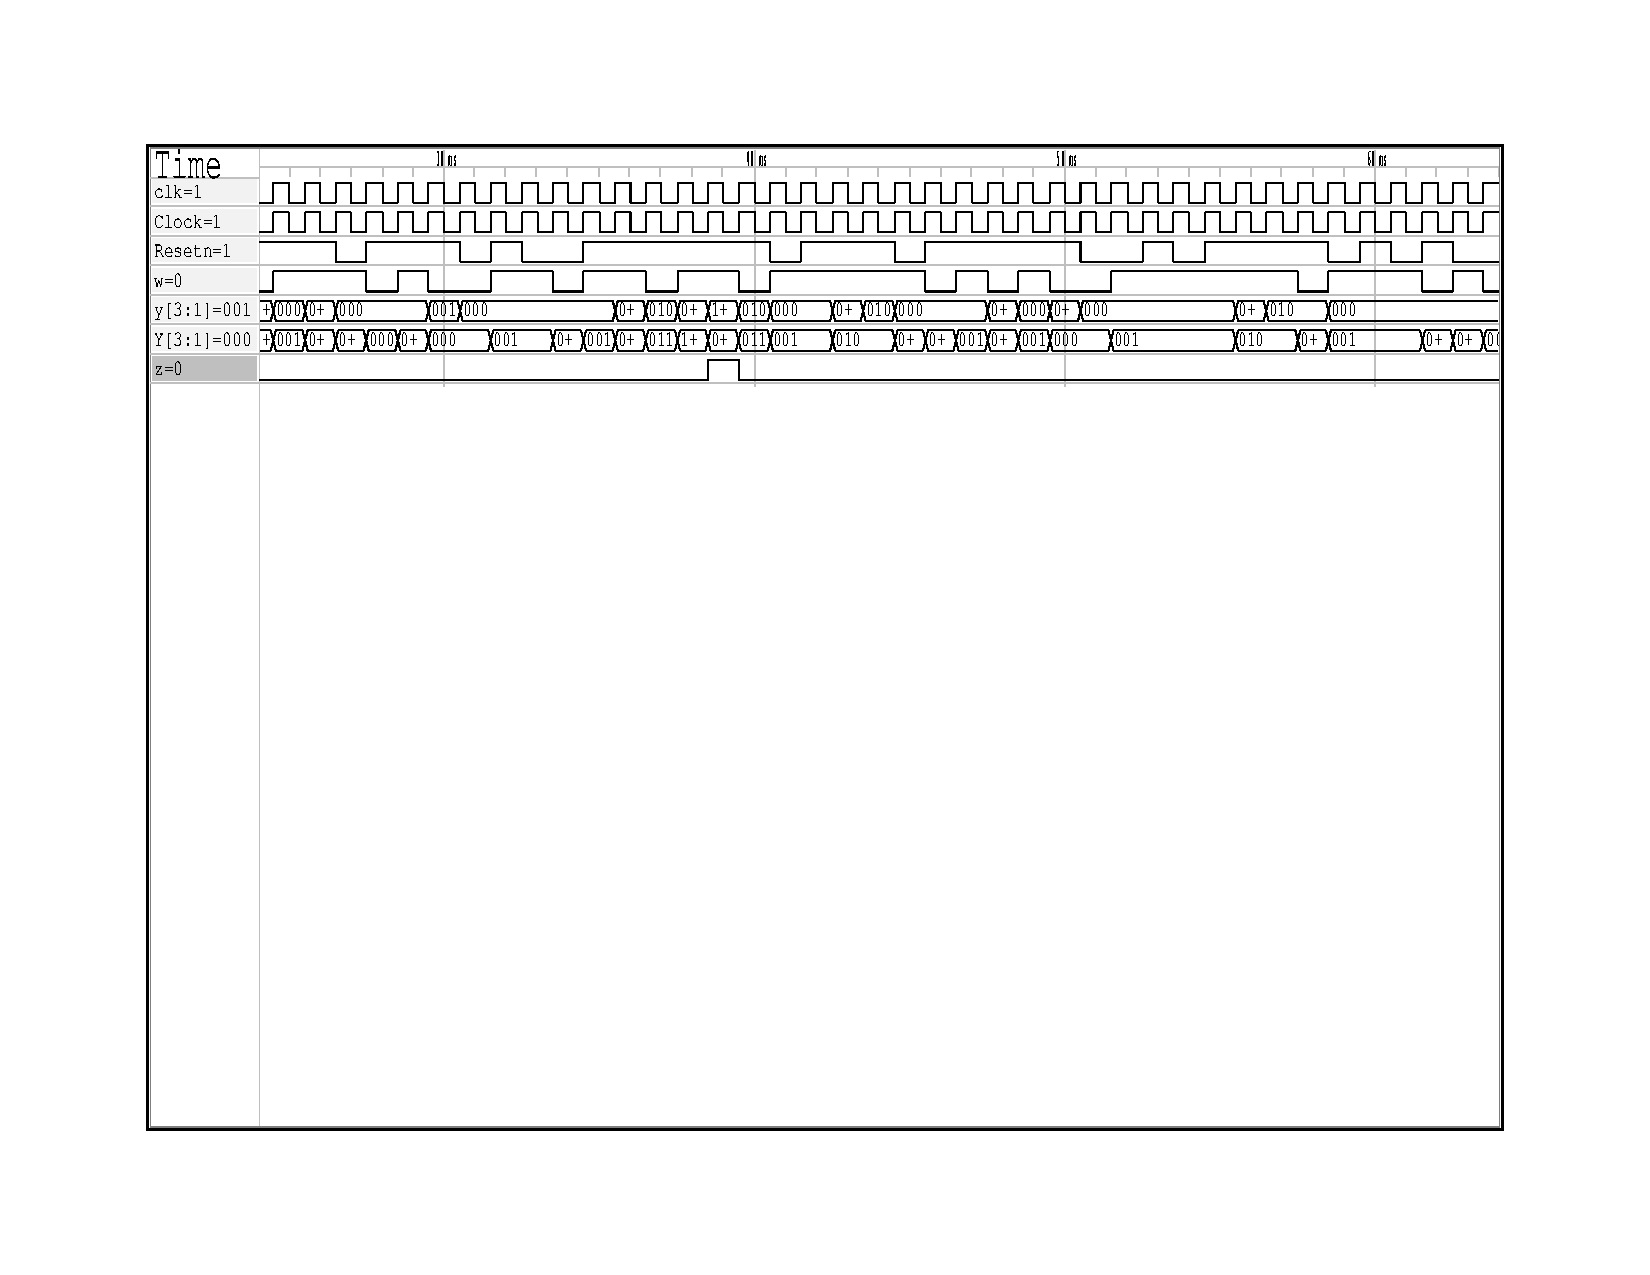
\includegraphics[scale=0.9]{../Exercise2/Moore/gtkr2}
\caption{\color{cyan}Test of reset in Moore's State Machine.}
\label{gtkr}
\end{figure}

In the previous figures \ref{gtk} and \ref{gtkr}, as previously mentioned, w is the input, y is the present states' vector, Y the next state's vector and z the output. It can be seen that the states' transition works correctly according to the input and to the reset signals. The output is 1 when the sequence 1-1-0-1 is detected.

%%
\subsection{\color{purple}Mealy Type State Machine}

In figure \ref {MealyEFSM} it is represented the sequence detection with the Mealy's state machine.

\begin{figure}[H]
\centering
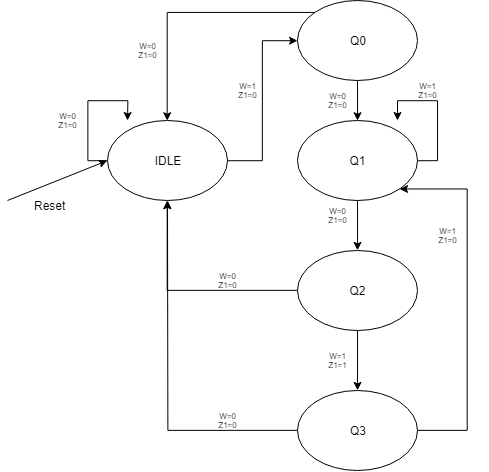
\includegraphics[scale=0.5]{../Exercise2/EJ2MEALY}
\caption{\color{cyan}Mealy's State Machine, for detecting the sequence 1-1-0-1.}
\label{MealyEFSM}
\end{figure}

It can be seen how in this case, the transition between one state to another now also causes a change in the output. It doesn't wait to get to the new state in order to change it. The following table is obtained from above's diagram in figure \ref {measej2} .

\begin{table}[H]
\begin{center}
\begin{tabular}{|c|c c c|c c c|}
\hline
Present State & & Next State & & & Output z & \\
 &  & depending on w& & & depending on w&  \\
 & w=0 & & w=1 & w=0& &w=1  \\
\hline
\hline
A (000)& A (000)& & B (001)& 0 & & 0   \\
\hline
B  (001)& A (000)& & C  (010)& 0 & & 0   \\
\hline
C (010)& D (011)& & C  (010)& 0 & & 0 \\
\hline
D (011)& A (000)& & E (100) & 0 & & 1  \\
\hline
E (100)& A (000)& & C  (010)& 0 & & 0 \\
\hline
\hline
\end{tabular}
\end{center}
\caption{\label{measej2}\color{cyan}Mealy's Next States and Outputs.}
\end{table}

\subsubsection{\color{orange}Coding and testing of the Mealy's State Machine}
The same tests with the same input sequences used for Moore's state machine, were used to test the Mealy's state machine. The results are seen in figures \ref{gtkk} and \ref{gtkrr}.


\begin{figure}[H]
\centering
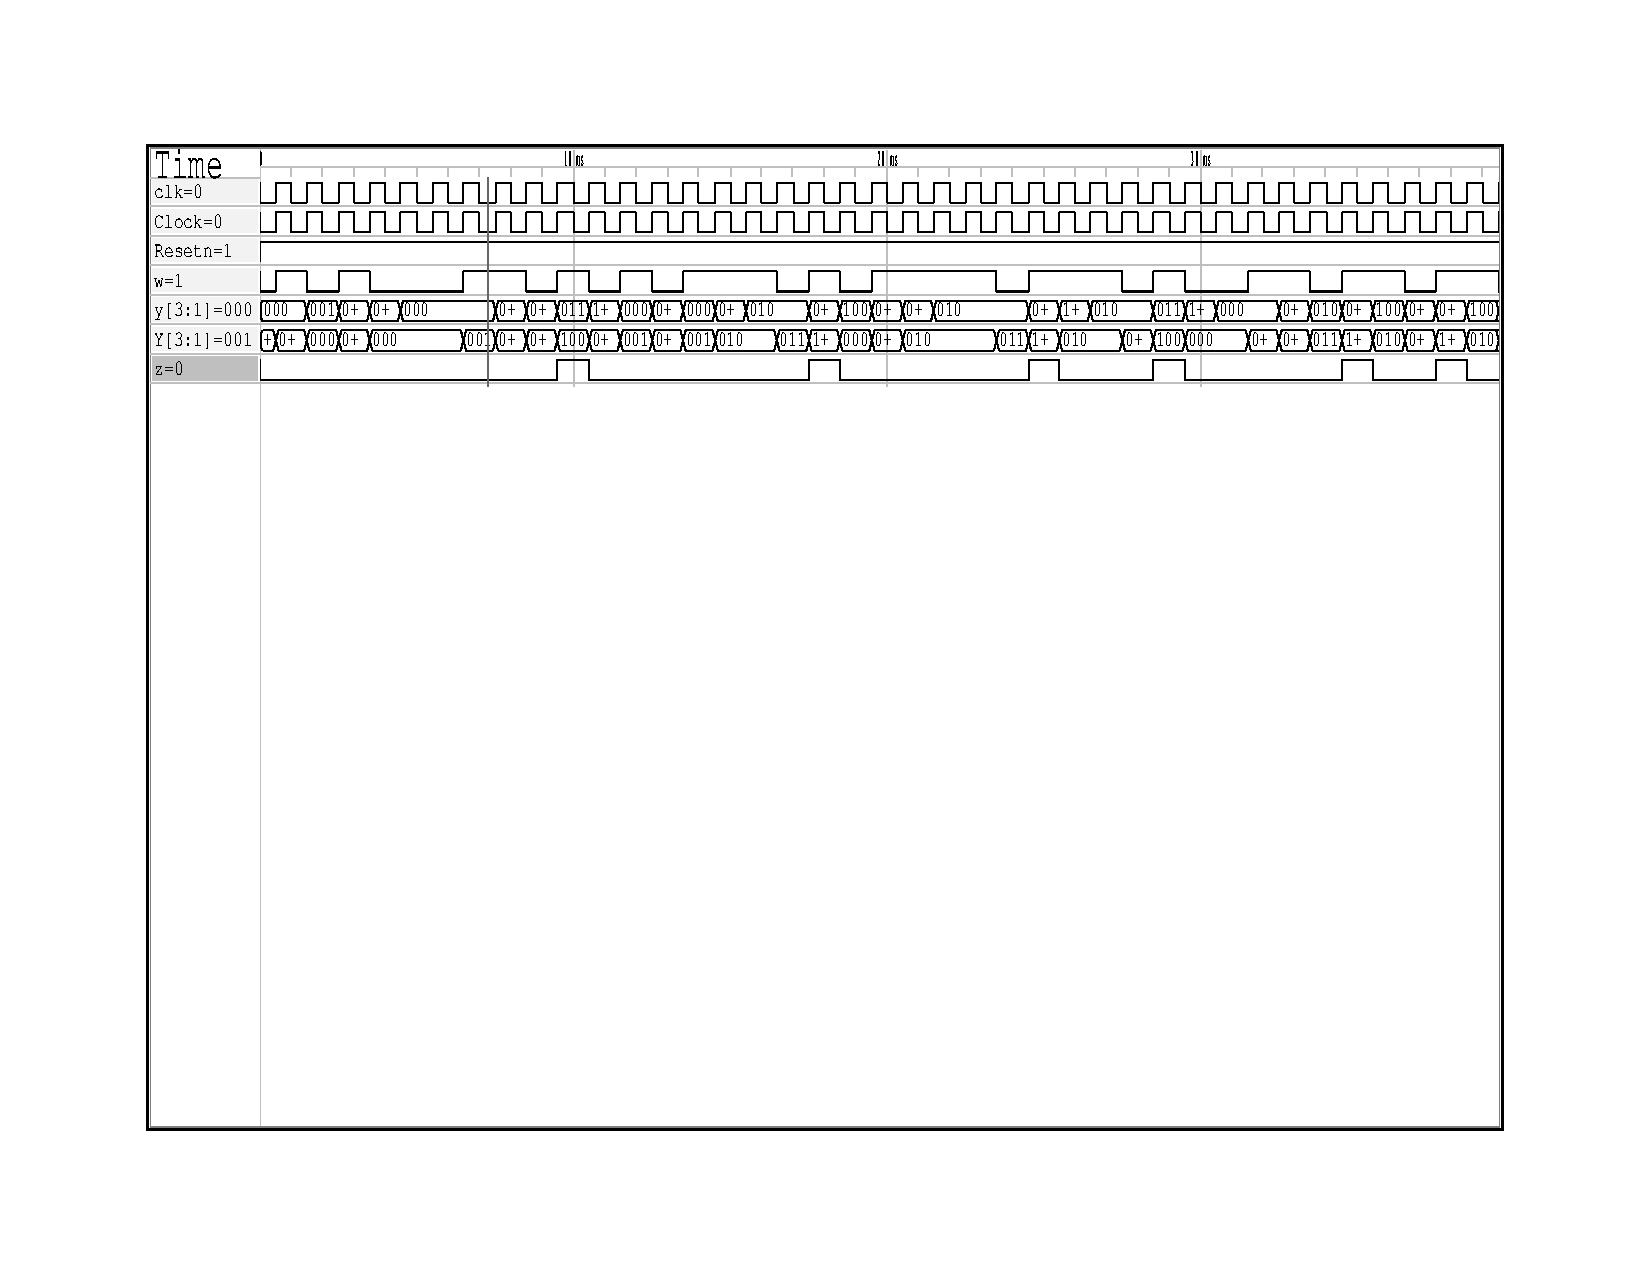
\includegraphics[scale=0.9]{../Exercise2/Mealy/gtk00}
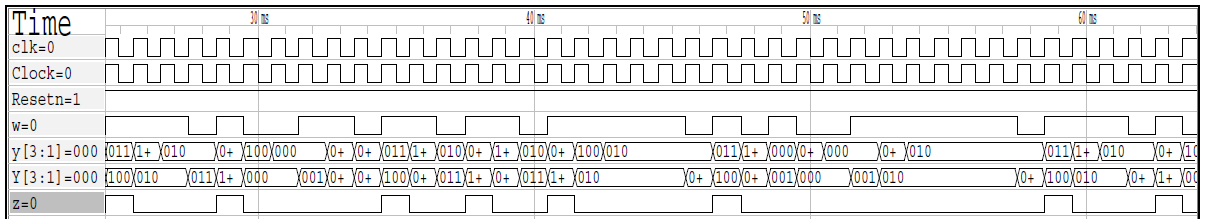
\includegraphics[scale=0.9]{../Exercise2/Mealy/gtk}
\caption{\color{cyan}Test of Moore's State Machine without resetting.}
\label{gtkk}
\end{figure}

\begin{figure}[H]
\centering
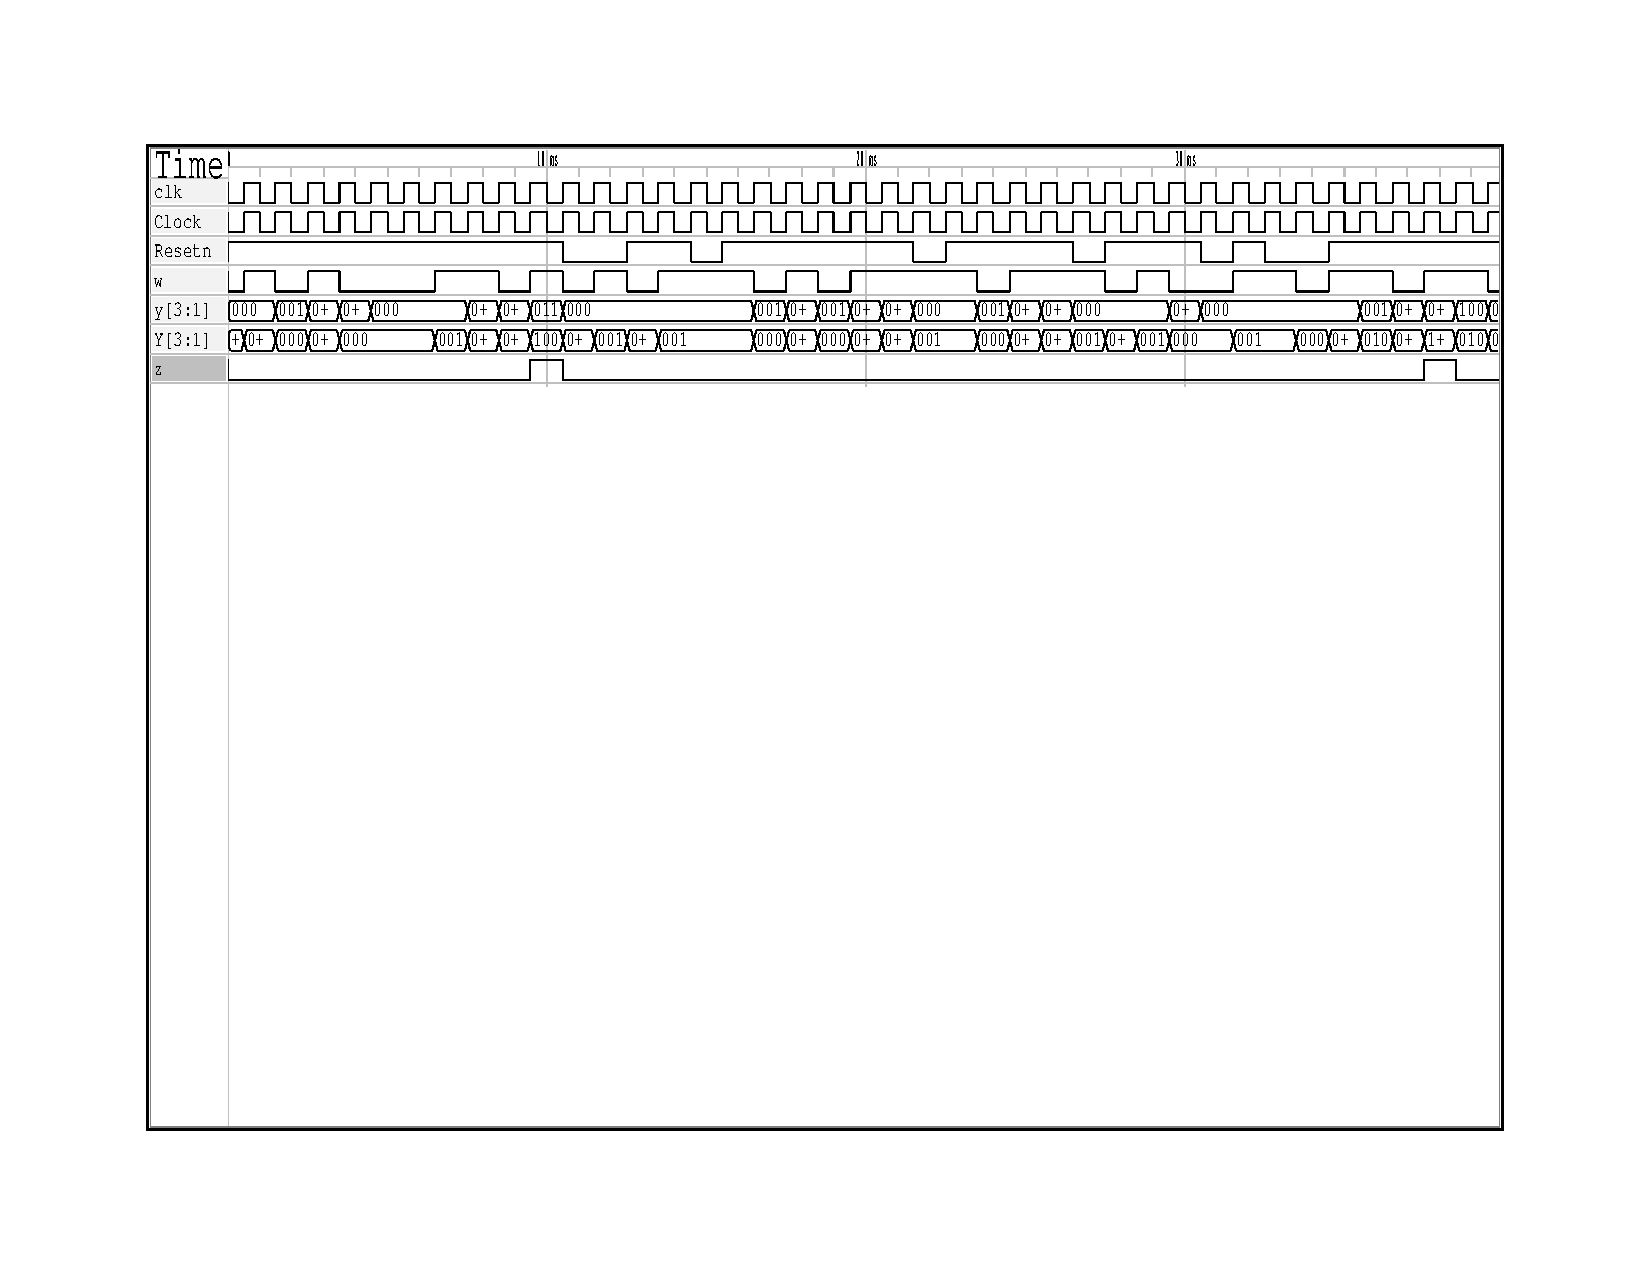
\includegraphics[scale=0.9]{../Exercise2/Mealy/gtkr1}
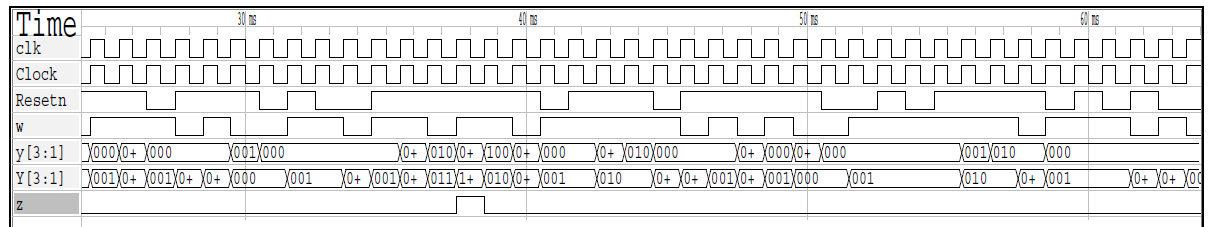
\includegraphics[scale=0.9]{../Exercise2/Mealy/gtkr2}
\caption{\color{cyan}Test of reset in Moore's State Machine.}
\label{gtkrr}
\end{figure}

As well as in the previous case, it can be seen that the Mealy's state machine works correctly according to the input w and to the reset signals. 

\subsubsection{\color{orange}Comparison of Moore's State Machine with Mealy's State Machine}
Even though both state machines work as expected and although they both answer correctly to the changes of states, in the gtkwave simulations it can be clearly seen the difference between the effect that each of the state machines have on the output z. In Moore's case, the output is high one clock after the sequence finishes appearing through the input. However, this one-clock delay doesn't happen in Mealy's State Machine. In the second one, the output doesn't only depend on the present state, but also on the input signal when going from one state to another. So the output is seen immidiatly when the last bit of the input signal arrives. This means that the Moore's output signal is the same as Mealy's one, but occuring one clock later.
